\documentclass[sigplan]{acmart}\settopmatter{printfolios=true,printccs=false,printacmref=false}
\usepackage{flushend}

\acmConference[PL'18]{ACM SIGPLAN Conference on Programming Languages}{January 01--03, 2018}{New York, NY, USA}
\acmYear{2018}
\acmISBN{} % \acmISBN{978-x-xxxx-xxxx-x/YY/MM}
\acmDOI{} % \acmDOI{10.1145/nnnnnnn.nnnnnnn}
\startPage{1}
\setcopyright{none}

\bibliographystyle{ACM-Reference-Format}

\begin{document}
\title{Wrattler: \textnormal{Reproducible, live and polyglot notebooks}}

\author{Tomas Petricek}
\affiliation{
  \institution{The Alan Turing Institute}
}
\email{tomas@tomasp.net}
\author{Charles Sutton}
\affiliation{
  \institution{The University of Edinburgh}
}
\additionalaffiliation{
  \institution{The Alan Turing Institute and Google}
}
\email{csutton@inf.ed.ac.uk}
\author{James Geddes}
\affiliation{
  \institution{The Alan Turing Institute}
}
\email{jgeddes@turing.ac.uk}

\definecolor{cmtclr}{rgb}{0.0,0.6,0.0}
\definecolor{kvdclr}{rgb}{0.0,0.0,0.6}
\definecolor{numclr}{rgb}{0.0,0.4,0.0}
\definecolor{strclr}{rgb}{0.4,0.4,0.0}
\definecolor{rstrclr}{rgb}{0.5,0.1,0.0}
\definecolor{prepclr}{rgb}{0.6,0.0,0.2}
\newcommand{\vect}[1]{\langl #1 \rangl}
\newcommand{\langl}{\begin{picture}(4.5,7)
\put(1.1,2.5){\rotatebox{60}{\line(1,0){5.5}}}
\put(1.1,2.5){\rotatebox{300}{\line(1,0){5.5}}}
\end{picture}}
\newcommand{\rangl}{\begin{picture}(4.5,7)
\put(.9,2.5){\rotatebox{120}{\line(1,0){5.5}}}
\put(.9,2.5){\rotatebox{240}{\line(1,0){5.5}}}
\end{picture}}
\newcommand{\ball}[1]{\FPeval{\result}{clip(201+#1)}\textnormal{\ding{\result}}}
\newcommand{\lsep}{~\,|\,~}
\newcommand{\num}[1]{\textcolor{numclr}{#1}}
\newcommand{\str}[1]{\textnormal{\textcolor{strclr}{\sffamily "#1"}}}
\newcommand{\strf}[1]{\textnormal{\textcolor{strclr}{\sffamily #1}}}
\newcommand{\rstr}[1]{\textnormal{\textcolor{rstrclr}{\sffamily "#1"}}}
\newcommand{\ident}[1]{\textnormal{\sffamily #1}}
\newcommand{\qident}[1]{\textnormal{\sffamily \textquotesingle #1\textquotesingle}}
\newcommand{\dom}{\ident{dom}}
\newcommand{\kvd}[1]{\textnormal{\textcolor{kvdclr}{\sffamily #1}}}

\newcommand{\bndclr}[1]{\textcolor{kvdclr}{#1}}
\newcommand{\bkndclr}[1]{\textcolor{prepclr}{#1}}
\newcommand{\blblclr}[1]{\textcolor{numclr}{#1}}
\newcommand{\bnd}[1]{\textnormal{\textcolor{kvdclr}{\sffamily #1}}}
\newcommand{\bknd}[1]{\textnormal{\textcolor{prepclr}{\sffamily #1}}}
\newcommand{\blbl}[1]{\textnormal{\textcolor{numclr}{\sffamily #1}}}

\begin{abstract}
Notebook systems such as Jupyter became a popular programming environment for data science, because 
they support interactive data exploration and provide a convenient way of interleaving code, 
comments and visualizations. However, most notebook systems use an architecture that makes
reproducibility and versioning difficult and limits the interaction model.

In this paper, we present Wrattler, a new notebook system built around provenance that addresses
the above issues. Wrattler separates state management from script evaluation and controls the 
evaluation using a dependency graph maintained in the web browser. This allows richer forms of 
interactivity, an efficient evaluation through caching, guarantees reproducibility and makes it 
possible to support versioning.
\end{abstract}
\keywords{notebook, dependency graph, live coding, AI}
\maketitle

\section{Introduction}
Notebooks \cite{ipython,jupyter} are literate programming \cite{literate} develoment
environments that allow data analyst to combine text, code and code outputs. Notebooks make
it easy to run code and see results. To further aid reproducible, iterative and exploratory data 
science, notebook systems should also support:

\paragraph{Richer interaction model.}
Web browsers are increasingly powerful and allow moving parts of data exploration to the client-side. 
Simple code changes should be evaluated efficiently using a cache and notebooks
should give live previews when writing code to perform simple data exploration.

\paragraph{Transparent state management.}
The state maintained by a notebook should be transparent and accessible to external tools. This
would allow versioning of state and development of tools to explore and manipulate the notebook state.

\paragraph{Multiple languages and tools.} 
A notebook should make it easy to combine multiple programming languages. A cell written in one
language should be able to automatically access data frames defined in other languages.

\paragraph{Improved reproducibility.} 
Changing code in a cell should invalidate results that depend on data frames defined in 
the cell. Reverting a change should immediately revert the result to the previous one
and show it immediately using a cache.

\newpage
~

\noindent
In this paper, we present Wrattler, a new notebook system that supports
the above features. We follow a line of work combining provenance tracking with notebooks 
\cite{noworkflow,dataflow}, but rather than extending existing systems, we revisit
two key aspects of the notebook architecture (Section~\ref{sec:arch}). 

First, Wrattler uses a \emph{dependency graph} to track provenance between cells and even function calls 
inside individual cells (Section~\ref{sec:comp-deps}). When a cell is changed, relevant parts of a graph
are invalidated. This guarantees reproducibility and enables more efficient re-computation.
Second, Wrattler introduces a \emph{data store} that separates state management from code execution 
(Section~\ref{sec:comp-data}). The data store handles versioning and simplifies the support for polyglot programming.

Together, these two changes to the standard architecture of notebook systems make Wrattler notebooks
(Section~\ref{sec:results}) polyglot, reproducible (with an easy and reliable state rollback) and live 
(with efficient re-computation on change that enables live preview during data exploration).

\begin{figure}[b]
\vspace{-1em}
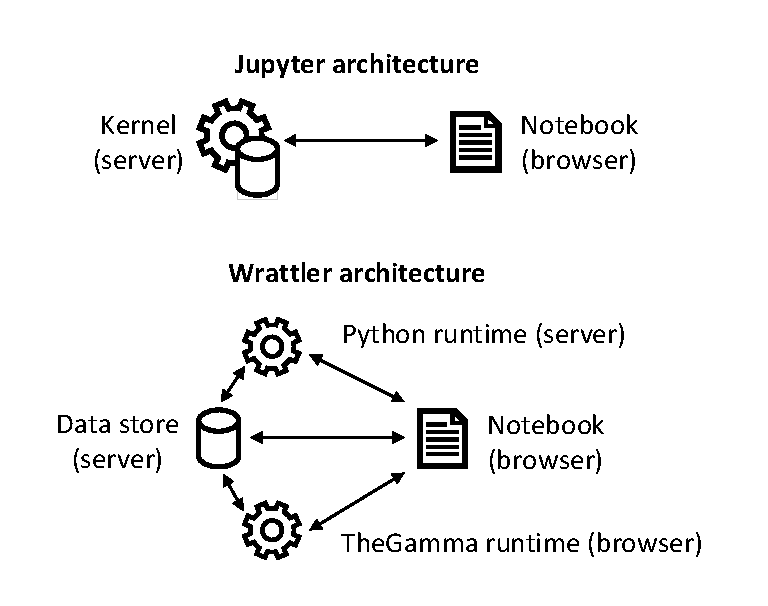
\includegraphics[scale=0.6]{diagram.pdf}
\vspace{-0.5em}
\caption{\small{In notebook systems such as Jupyter, state and execution is managed by a kernel. In
  Wrattler, those functions are split between data store and language runtimes. Language runtimes 
  can run on the server-side (e.g.~Python) or client-side (e.g.~TheGamma).}}
\label{fig:arch}
\end{figure}

\section{Wrattler architecture}
\label{sec:arch}
Standard notebook architecture consists of a \emph{notebook} and a \emph{kernel}. The kernel
runs on a server, evaluates code snippets and maintains state they use.
Notebook runs in a browser and sends commands to the kernel in order to evaluate 
cells selected by the user. As illustrated in Figure~\ref{fig:arch}, Wrattler splits the 
server functionality between two components:

\paragraph{Data store.} Imported external data and results of running scripts  
are stored in the data store. The data store keeps version history and annotates data with 
metadata such as types, inferred semantics and provenance information.

\paragraph{Language runtimes.} Code in notebook cells is evaluated by language runtimes.
The runtimes read input data from and write results back to the data store. Wrattler supports
language runtimes that run code on the server (similar to Jupyter kernels), but also language
runtimes that parse and evaluate code directly in the browser.

\paragraph{Notebook.} The notebook is displayed in a web browser and orchestrates 
all other components. The browser builds a dependency graph between cells or individual 
calls. It invokes language runtimes to evaluate code that has changed,
and reads data from the data store to display results.  

\section{Wrattler components}
\label{sec:comp}

Wrattler consists of a notebook user interface running in the web browser, which communicates 
with the data store and multiple server-side language runtimes. We also provide an integration 
with a simple data exploration language TheGamma \cite{thegamma} that has a fully client-side language
runtime. 

\subsection{TheGamma script}
\label{sec:comp-gamma}

The Wrattler architecture supports languages that require running a separate language runtime
as a server, but also languages that can be parsed and evaluated in the browser. To illustrate this, 
we integrated Wrattler with TheGamma~\cite{thegamma}, a simple browser-based language 
for data exploration.

As an example, we use a data set with broadband speed published by the UK government \cite{ofcom}.
The following script written using TheGamma loads the online CSV file, groups rows by whether they represent
rural or urban area and then calculates average download speed for both area kinds:

\noindent
\begin{equation*}
\hspace{-3em}
\begin{array}{l}
\ident{web.loadTable}(\str{https://.../bb2014.csv}).\ident{explore}.\\
\quad\qident{group data}.\qident{by Urban/rural}.\\
\qquad\qident{average Download speed (Mbit/s) 24 hrs}  
\end{array}
\end{equation*}

\noindent
Identifiers such as \qident{by Urban/rural} are generated by a \emph{type provider} \cite{providers} 
and the user typically interacts by selecting one of generated members through an auto-complete
(hence the long explicity names are acceptable). For the purpose of this paper, the most 
important aspect is that TheGamma scripts can be parsed, checked and evaluated in the browser.

\subsection{Dependency graph}
\label{sec:comp-deps}

When opening a notebook, Wrattler parses the source of the notebook (consisting of text cells and
code cells) and constructs a dependency graph, which serves as a runtime representation of the
notebook. The parsing of code cells is done by language runtimes that parse and statically analyse 
code and constructs parts of the dependency graph.

Wrattler uses a \emph{data frame} as a primary format for passing data between cells.
Data frames represent tables with multiple (named) columns and (anonymous) rows. Data frames
have a first-class support in most data science languages.

\begin{figure}
\vspace{-0.5em}
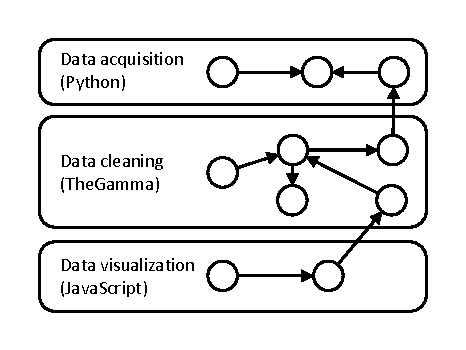
\includegraphics[scale=1,trim=0.5cm 0.5cm 0.5cm 0.5cm]{graph.pdf}
\vspace{-0.5em}
\caption{\small{Dependency graph of a sample notebook with three cells. The cells are written
in Python, Wrattler script and JavaScript. The browser builds a fine-grained dependency graph
for Wrattler script that can be parsed and analysed in the browser.}}
\label{fig:deps}
\vspace{-1em}
\end{figure}

As an example, consider a simpler notebook with three cells. The first cell, written in Python,
downloads data and exports the result as a data frame; the second cell is written in TheGamma script
and performs data cleaning and the third cell creates a visualization in JavaScript. The
resulting dependency graph is shown in Figure~\ref{fig:deps}.

Wrattler creates two nodes for each cell, representing the cell as a whole and its source
code. In addition, it creates a node for each data frame exported by a cell (e.g.~the rightmost
node in the first cell). Code in subsequent cells can depend on data frames exported from earlier
cell, which is captured as a dependency in the graph. 

The dependency graph is updated after each code change and so it needs to be constructed efficiently 
in the browser. Language runtime that run on the client-side create a more fine-grained 
dependency graph with a node for each operation (such as member access or a function call). This 
is the case in the  second cell in Figure~\ref{fig:deps}. This allows live update of results when 
code changes as we only need to re-evaluate small parts of code in a cell. 

\paragraph{Dependency graph construction.} 
The dependency graph is updated after every code change. Wrattler first parses each 
cell, producing a single syntactic element for Python and JavaScript cells (representing the entire 
source code) and a syntax tree for TheGamma (representing member accesses and other 
constructs). The syntax tree for the entire notebook is then a list of elements produced for each 
cell.
 
After parsing, Wrattler walks over the syntax tree recursively and binds a dependency graph node
to each syntactic element in the tree using a process decribed in Figure~\ref{fig:bind}. 
The \emph{antecedents} of a node are the nodes that it depends on. This typically includes 
inputs for an operation or instance on which a member access is performed. 

\paragraph{Checking and evaluation.} 
Nodes in the dependency graph can be annotated with information such as the evaluated value
of the syntactic element that the node represents. An important property of the binding process
(Figure~\ref{fig:bind}) is that, if there is no change in antecedents of a node, binding will 
return the same node as before. This means that if we evaluate a value for a given node in a 
dependency graph and attach it to a node, the value will be cached and reused. 

Wrattler re-evaluates parts of the dependency graph on demand and the displayed results and 
visualizations always reflect the current source code in the notebook. When the evaluation 
of a cell is requested, Wrattler recursively evaluates all the antecedents of the node and 
then evaluates the value of the node. The evaluation is delegated to a language
runtime associated with the language of the node:
%
\begin{enumerate}
\item For Python nodes, the language runtime sends the source code, together with its 
  dependencies, to a server that retrieves the dependencies and evaluates the code.
\item For TheGamma and JavaScript nodes, the language runtime collects values of the 
  dependencies and runs the operation that the node represents in the browser.
\end{enumerate}
%
Wrattler also uses the dependency graph for type checking. Just like evaluation, type checking
is done by recursively walking over the dependency graph and annotating the nodes with their 
type. This step is only relevant for cells written in statically typed languages, but it provides
a quick feedback, because it does not need to evaluate the code.

\subsection{Data store}
\label{sec:comp-data}

The data store enables communication between individual Wrattler components and provides a way for 
persistently stroing input data. It stores raw input data, data frames and multiple versions of the 
dependency graph. Data frames stored in the data store are associated with the hash produced by the 
binding process outlined in Figure~\ref{fig:bind} and are immutable. When the notebook changes, 
new nodes with new hashes are created. New data frames are appended, rather than overwriting 
existing state.

External input data files imported into Wrattler notebooks (such as downloaded web pages) are 
stored as binary blobs. Data frames are currently stored in JSON format (as an array of records),
but we intend to use a suitable database system in the future. Data frames are used for
communication between multiple cells of a Wrattler notebook. To make a data frame available to 
subsequent cells, a cell can export and store a data frame into the data store (the
key is the hash of the node representing the data frame). 

The data store also supports a mechanism for annotating data frames with 
semantic information. Columns can be annotated with primitive data type such as 
date or floating-point number. Columns can be annotated with semantic annotation that indicates
the meaning of the column -- for example, address or longitude and latitude. Finally, columns,
rows and individual cells of the data frame can be annotated with other metadata such as their
data source.

\begin{figure}
\vspace{-1em}
\begin{equation*}
\hspace{-6em}\begin{array}{l}
\kvd{procedure}~\ident{bind}(\textit{cache}, \textit{syn})~=\\
\quad \kvd{let}~h = \{ \ident{hash}(\ident{kind}(\textit{syn})) \} \\  
\quad \qquad \cup~ \{\ident{hash}(c) \,|\, c\in\ident{antecedents}(\textit{syn}) \}\\
\quad \kvd{if}~\ident{not}~\ident{contains}(\textit{cache}, h)~\kvd{then}\\
\quad \quad \kvd{let}~n = \emph{fresh node}\\
\quad \quad \ident{value}(n) \leftarrow \ident{Unevaluated} \\
\quad \quad \ident{hash}(n) \leftarrow h\\
\quad \quad \ident{set}(\textit{cache}, h, n) \\
\quad \ident{lookup}(\textit{cache}, h)\\
\end{array}
\end{equation*}
\vspace{-0.5em}
\caption{\small{When binding a graph node to a syntactic element, Wrattler first computes
  a set of hashes that uniquely represent the node. This includes hash of the kind of the 
  node (e.g. the source code of a Python node or member name in TheGamma) and hashes
  of all antecedents. If a node with a given hash does not exist in cache, a new node
  is created. We set its hash, indicate that its value has not been evaluated and
  add it to the cache.}}
\label{fig:bind}
\end{figure}

In addition to storing the raw data, the data store also persistently stores the current and
multiple past versions of the dependency graph constructed from the notebook (saved by an 
explicit checkpoint). This makes it possible to analyse the history of a notebook and track how
data is transformed by the computation in a notebook.

\subsection{Third-party tools}
\label{sec:comp-ai}

The Wrattler architecture enables integration of third-party tools that analyse the notebook
or data it uses and provide hints to the data analyst. Most notably, such tools include AI 
assistants that help with tedious data cleaning and pre-processing tasks. 

As an example, datadiff \cite{datadiff} is an AI assistant that reads two specified data frames from the
data store and suggests a script that transforms the data in the second data frame to match the
format of the first data frame. The AI assistant does not automatically transofrm the data, but
instead, produces a new cell in TheGamma script that can be reviewed by the data analyst. 
For example:
%
\begin{equation*}
\begin{array}{l}
\ident{datadiff(broadband2014, broadband2015)}\\
\quad.\ident{drop\_column}(\str{WT\_national})\\
\quad.\ident{drop\_column}(\str{WT\_ISP})\\
\quad.\ident{recode\_column}(\str{URBAN}, [\num{1}, \num{2}], [\str{Urban},\str{Rural}])
\end{array}  
\end{equation*}
%
The script specifies that two columns should be dropped from the corrupted second data frame and
one column needs to be recoded (turning $\num{1}$ and $\num{2}$ into strings
\strf{Urban} and \strf{Rural}). 

\section{Properties of Wrattler}
\label{sec:results}

The Wrattler architecture outlined in Section~\ref{sec:arch} leads to a number of properties that
are difficult to obtain with traditional notebook systems. In this section, we discuss the 
properties and briefly discuss our prototype implementation.

\subsection{Reproducible, live and smart}
The two most important aspects of the Wrattler architecture are that it separates the state from 
the language runtime (using a data store) and that it keeps a dependency graph based on the current
notebook source code (on the client). The provenance information that is available thanks to this
arhcitecture enable a number of properties.

\paragraph{Reproducibility.} The evaluation outputs displayed in Wrattler notebook always reflect
the current source code. When code changes, Wrattler updates the dependency graph and hides 
invalidated visualizations. Because the data store caches earlier results, it is always possible
to go back without re-evaluating the whole notebook.

\paragraph{Refactoring.} The dependency graph allows us to implement notebook refactoring. 
For example, it is possible to extract only code necessary to produce a given visualization.
For code written in TheGamma, this extracts individual operations; for Python or JavaScript,
we can currently extract code at cell-level granularity.

\paragraph{Live previews.} The dependency graph makes it possible to give 
live previews during development. When code changes, only values for new nodes in the graph 
need to be calculated. The fine-grained structure of the dependency graph for TheGamma 
makes it possible to update previews instantly.

\paragraph{Polyglot.} Sharing the state via data store makes it possible to combine multiple
langauge runtimes, as long as they support sharing data via data frames. In our prototype, this
includes R, JavaScript and TheGamma script, but the extensibility model allows adding further
languages.

\subsection{Wrattler prototype}

A prototype implementation of the Wrattler system is available on GitHub (\url{http://github.com/wrattler}).
The prototype implements language runtimes for JavaScript, TheGamma script and R 
(Section~\ref{sec:comp-gamma}). It builds a dependency graph (Section~\ref{sec:comp-deps})
and uses it to evaluate results of cells. 

The data store (Section~\ref{sec:comp-data}) 
stores data in Microsoft Azure in JSON format. Support for meta-data annotations and big data
is not yet implemented. The protoype comes with one third-party tool -- the datadiff AI 
assistant mentioned above (Section~\ref{sec:comp-data}). Figure~\ref{fig:proto} shows the 
first cell of a sample Wrattler notebook analysing the UK broadband data.

\begin{figure}
\vspace{-0.5em}
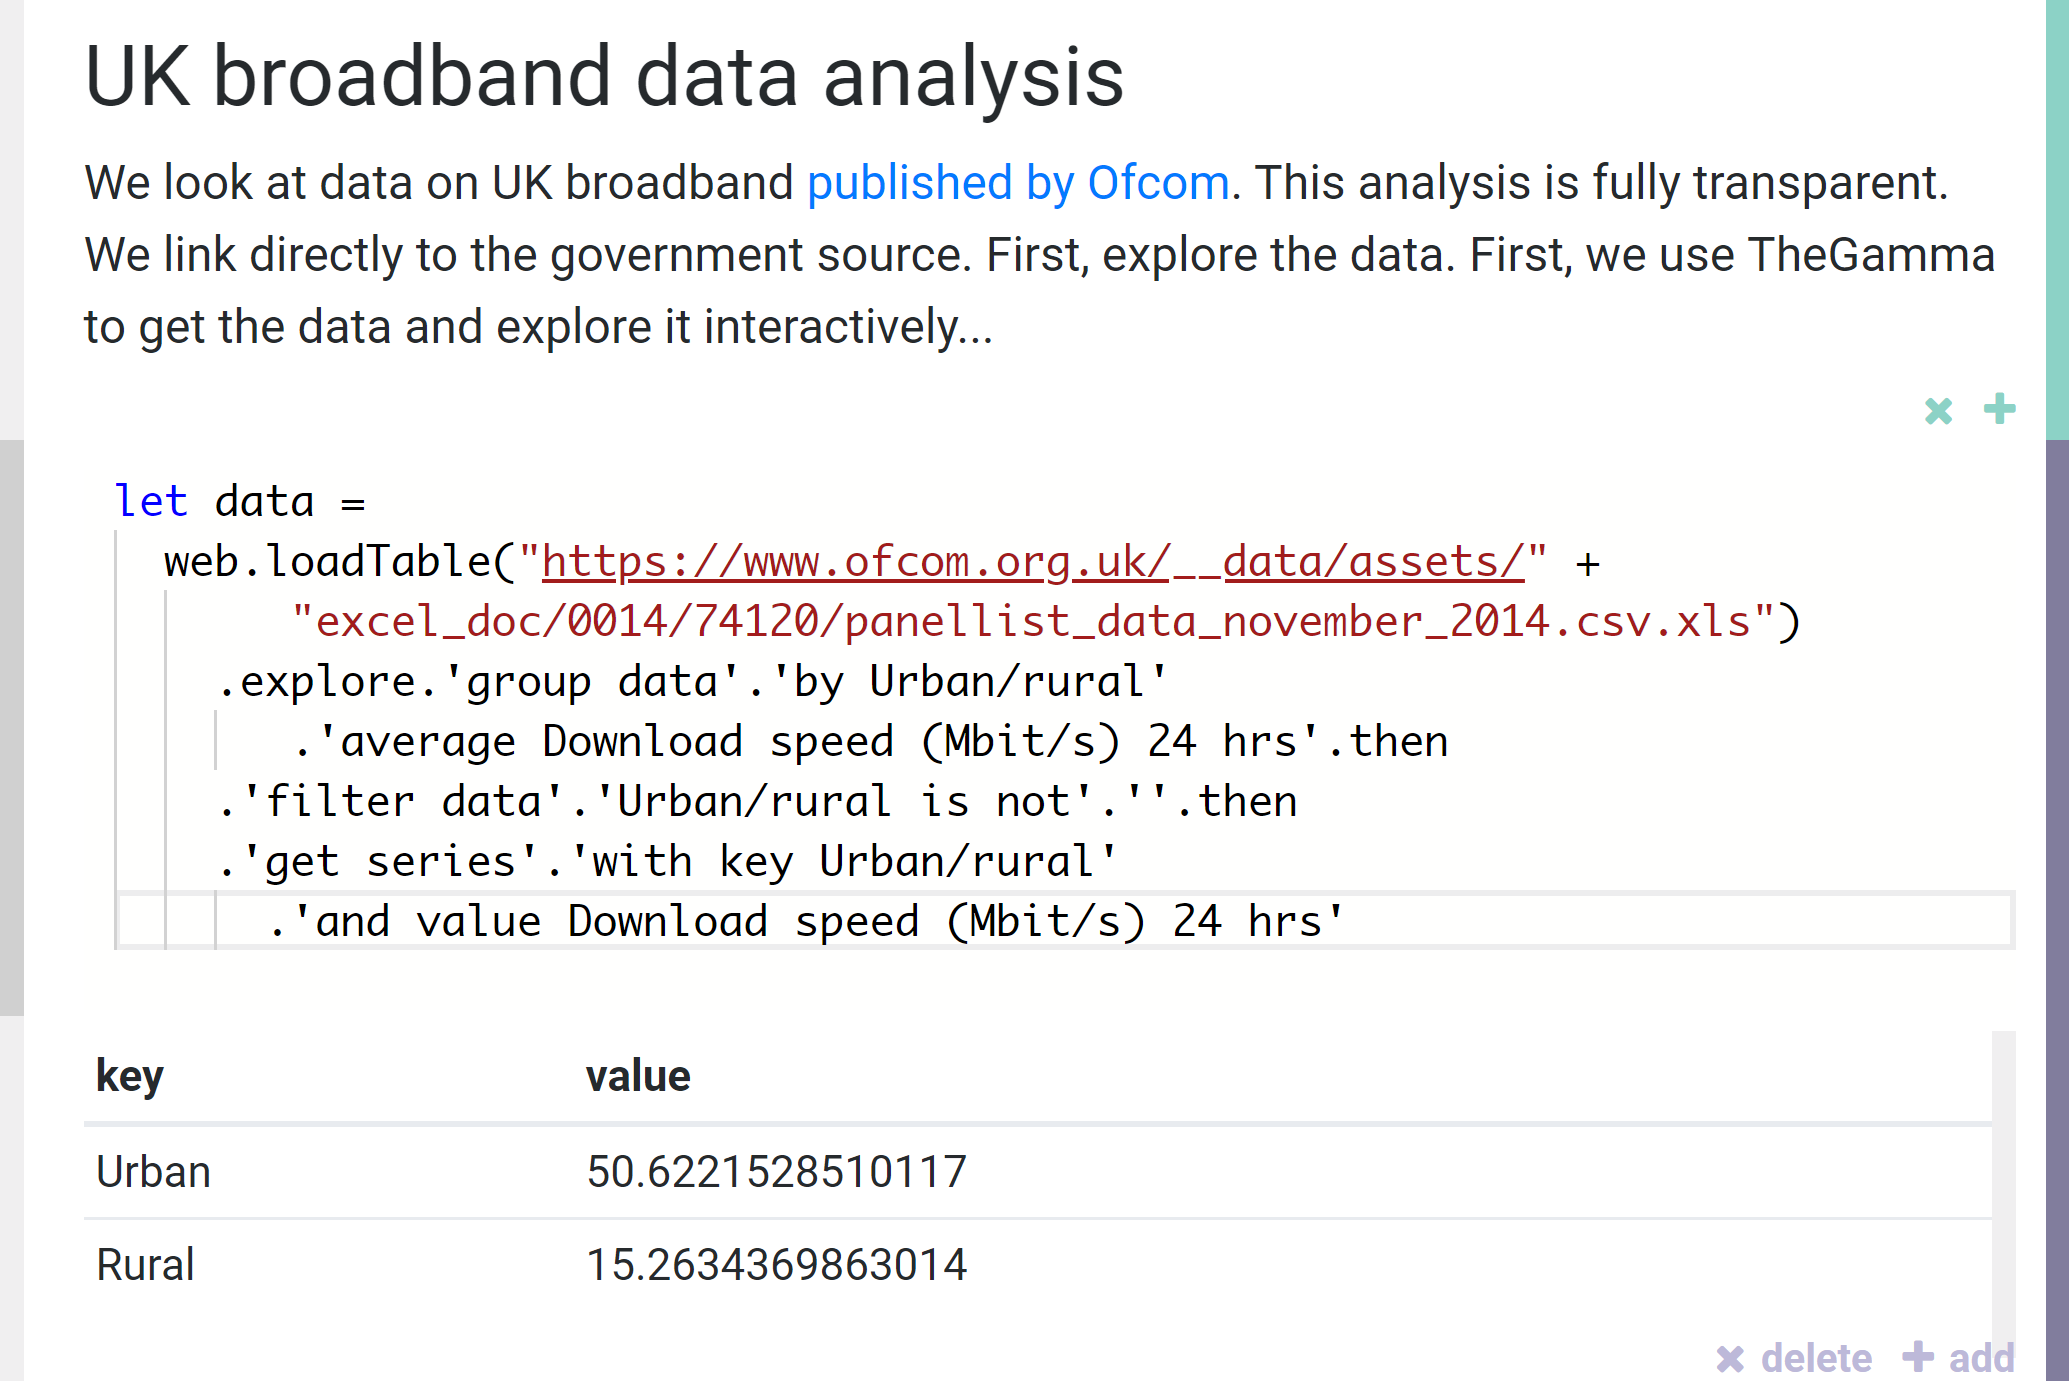
\includegraphics[scale=0.15]{screen.png}
\caption{\small{TheGamma script that downloads and aggregates UK government data, running in 
  Wrattler notebook with a live preview.}}
\label{fig:proto}
\vspace{-0.5em}
\end{figure}

\section{Related work}

The work in this paper directly follows the work on IPython and Jupyter systems
\cite{ipython,jupyter}. Wrattler shares many properties with those and aims to address some
of their limitations. To address reproducibility, some Jupyter extensions and systems such
as R markdown \cite{rmarkdown} lock cells after evaluation. 

Dataflow notebooks \cite{dataflow} are attach unique hashes to cell 
evaluations. This allows the user to refer to dependencies explicitly and, in effect, construct
a dependecy graph similar to ours manually.
Scientific workflow systems \cite{taverna,kepler} manage evaluation of workflows over a 
dependency graph similarly to Wrattler, but often allow editing it directly via a GUI, rather
than through code in a notebook.

The noWorkflow project \cite{noworkflow} links the two approaches by instrumenting Jupyter 
kernel with a mechanism for capturing provenance based on light-weight annotations.
Vizer \cite{vizer} focuses on integrating notebooks with spreadsheet-like interface.
It internally uses a data store component similar to ours, but does not keep dependency graph
on the client.

Our dependency grpah construction is inspired by Roslyn \cite{roslyn} and extends an
earlier work on TheGamma \cite{livegamma}. It is simiar to methods used in live programming 
languages \cite{live,subtext}, incremental compilation \cite{incremental} and
partial evaluation \cite{partial}. Wrattler adapts those methods to a notebook environment. 

\section{Summary}

This paper presents early work on Wrattler -- a new notebook system for data science that makes
notebooks reproducible, live and polyglot. The properties of Wrattler are enabled by provenance
information that is maintained thanks to two changes to the standard architecture of notebook 
systems. 

First, Wrattler separates the state management from code execution. This allows versioning,
polyglot notebooks and integration of third-party tools that can work directly with
the data store. Second, Wrattler keeps a dependency graph on the client (web browser) and uses 
it to control evaluation. This guarantees reproducibility and allows faster feedback during
development.

\begin{acks}
We thank to our colleagues from the AIDA (Artificial Intelligence for data analytics) project
Chris Williams, Zoubin Ghahramani and Ian Horrocks and attendees of a recent 
AIDA workshop. This work was in part supported by The Alan Turing 
Institute under the EPSRC grant EP/N510129/1.
\end{acks}

\bibliography{paper}
\end{document}
